%\graphicspath{{./Plots/}}


\documentclass[conference]{IEEEtran}
%%%%%%%%%%%%%%%%%%%%%%%%%%%%%%%%%%%%%%%%%%%%%%%%%%%%%%%%%%%%%%%%%%%%%%%%%%%%%%%%%%%%%%%%%%%%%%%%%%%%%%%%%%%%%%%%%%%%%%%%%%%%%%%%%%%%%%%%%%%%%%%%%%%%%%%%%%%%%%%%%%%%%%%%%%%%%%%%%%%%%%%%%%%%%%%%%%%%%%%%%%%%%%%%%%%%%%%%%%%%%%%%%%%%%%%%%%%%%%%%%%%%%%%%%%%%
\usepackage{amssymb}
\usepackage{amsmath}
\usepackage{geometry}
\usepackage{graphicx}
\usepackage{amsfonts}

\setcounter{MaxMatrixCols}{10}
%TCIDATA{OutputFilter=LATEX.DLL}
%TCIDATA{Version=5.50.0.2960}
%TCIDATA{<META NAME="SaveForMode" CONTENT="1">}
%TCIDATA{BibliographyScheme=BibTeX}
%TCIDATA{Created=Wednesday, December 09, 2020 21:10:24}
%TCIDATA{LastRevised=Monday, December 14, 2020 14:56:08}
%TCIDATA{<META NAME="GraphicsSave" CONTENT="0">}
%TCIDATA{<META NAME="DocumentShell" CONTENT="Articles\SW\IEEE Transactions for Conferences">}
%TCIDATA{CSTFile=IEEEtran.cst}

\graphicspath{{c:/Users/lin11/OneDrive/Documents/JHU-DESKTOP-MR0GT8B/adversarial_examples/}}
\newtheorem{theorem}{Theorem}
\newtheorem{acknowledgement}[theorem]{Acknowledgement}
\newtheorem{algorithm}[theorem]{Algorithm}
\newtheorem{axiom}[theorem]{Axiom}
\newtheorem{case}[theorem]{Case}
\newtheorem{claim}[theorem]{Claim}
\newtheorem{conclusion}[theorem]{Conclusion}
\newtheorem{condition}[theorem]{Condition}
\newtheorem{conjecture}[theorem]{Conjecture}
\newtheorem{corollary}[theorem]{Corollary}
\newtheorem{criterion}[theorem]{Criterion}
\newtheorem{definition}[theorem]{Definition}
\newtheorem{example}[theorem]{Example}
\newtheorem{exercise}[theorem]{Exercise}
\newtheorem{lemma}[theorem]{Lemma}
\newtheorem{notation}[theorem]{Notation}
\newtheorem{problem}[theorem]{Problem}
\newtheorem{proposition}[theorem]{Proposition}
\newtheorem{remark}[theorem]{Remark}
\newtheorem{solution}[theorem]{Solution}
\newtheorem{summary}[theorem]{Summary}
\input{tcilatex}
\begin{document}

\title{Generating and defending against adversarial examples in
vision-optimized neural architectures}
\pubid{\copyright ~2020 }
\specialpapernotice{}
\date{December 9, 2020}

%TCIMACRO{%
%\TeXButton{Author Information}{\author{\authorblockN{Daniel Donoghue}
%\authorblockA{
%Email: ddonogh1@jhu.edu}
%\and
%\authorblockN{Nicholas Lines}
%\authorblockA{
%Email: nicholasalines@gmail.com}
%\and
%\authorblockN{Arnaldo Pereira}
%\authorblockA{
%Email: aepereira@gmail.com}
%}}}%
%BeginExpansion
\author{\authorblockN{Daniel Donoghue}
\authorblockA{
Email: ddonogh1@jhu.edu}
\and
\authorblockN{Nicholas Lines}
\authorblockA{
Email: nicholasalines@gmail.com}
\and
\authorblockN{Arnaldo Pereira}
\authorblockA{
Email: aepereira@gmail.com}
}%
%EndExpansion

%TCIMACRO{\TeXButton{Make Title}{\maketitle}}%
%BeginExpansion
\maketitle%
%EndExpansion

%TCIMACRO{\TeXButton{Begin abstract}{\begin{abstract}}}%
%BeginExpansion
\begin{abstract}%
%EndExpansion

As automated decision-making becomes more popular and more dependent upon
artificial intelligence, securing sensitive models from adversarial behavior
has become essential. Neural networks are particularly vulnerable to
so-called adversarial examples \cite{szegedy2014intriguing}, and various
attacks and defences have been explored in the literature.

Our intention in this paper is to demonstrate and confirm the results of
such attacks at an informative but modest scale. We apply two common attacks
to both the wide ResNet and GoogLeNet neural models, and test two defences,
in a reproducible computational environment. We show that significant
improvements in network robustness are available with minimal defence
measures.

The authors are listed alphabetically, and all made equal contributions.
This work is performed in association with the Johns Hopkins Engineering for
Professionals Program, as a project for EN.625.638.8VL2.FA20 Neural Networks.

All code and further reference materials are available online at
https://github.com/linesn/adversarial\_examples.

%TCIMACRO{\TeXButton{End abstract}{\end{abstract}}}%
%BeginExpansion
\end{abstract}%
%EndExpansion

%TCIMACRO{\TeXButton{Table of Contents}{\tableofcontents}}%
%BeginExpansion
\tableofcontents%
%EndExpansion

\bigskip

\section{Executive Summary}

Since 2014 when Szegedy et al \cite{szegedy2014intriguing} published the
first observation on the subject, adversarial examples have gained much
attention in both the study of adversarial machine learning research and the
more results-oriented world of practical neural archetecture, due to the
alarming weaknesses they expose and the interesting robustness that can be
introduced via defence efforts. The term "adversarial example" is used to
describe "an input to a machine learning model that is intentionally
designed to cause the model to make a mistake in its predictions, despite
resembling a valid input to a human" \cite{wiyatno2019adversarial}. As such
these examples are classed as evasion techniques by adversarial machine
learning theory, since their goal is to evade detection while producing
misinterpretations \cite{wiki:aml}.

Most of the literature on the subject (in keeping with traditions in the
neural network community) uses image recognition tasks to demonstrate the
efficacy of attacks and defences, and we will do the same. In this paper we
will demonstrate successful us of the Fast Gradient Sign Method (FGSM) \cite%
{goodfellow2014explaining} and Directed Gradient Sign (DGSM) \cite%
{madry2020adversarial} attacks against convolutional neural networks trained
with Imagenette data. We will then examine the results of applying two
common defences: first, perturbed prediciton averaging, and second, training
using adversarial examples. We confirm the observations of Goodfellow et al 
\cite{goodfellow2014explaining} and show that, while the Wide ResNet and
GoogLeNet architectures are very susceptible to the above attacks, the named
defences also produce significant improvement to the robustness of the
classifiers.

\section{Project overview}

\subsection{Why are adversarial examples effective?}

In practice neural architectures based on linear components are prefered
(over, for example, radial basis components) because of their speed in
training and inference. However, it is this property that makes them
particularly vulnerable to the most common form of adversarial example \cite%
{goodfellow2014explaining}. Neural classifier inputs or features naturally
have some precision limit, such as a color range or pixel count, below which
perturbations are ignored. Consider an input vector $\mathbf{X}$, to which
we add a noise vector $\mathbf{\eta }$, where every $\eta \in \mathbf{\eta }$
is smaller than $\epsilon ,$ the precision limit. To humans and a first pass
review by machines, $\mathbf{X}$ and $\mathbf{X+\eta }$ are identical.
However, when the linear activity function is computed, the network's
weights are dotted with the input, yielding approximately 
\begin{equation*}
\mathbf{W}^{\intercal }(\mathbf{X+\eta )=W}^{\intercal }\mathbf{X+W}%
^{\intercal }\mathbf{\eta ,}
\end{equation*}%
where the noise term $\mathbf{W}^{\intercal }\mathbf{\eta }$ can grow very
large if $\mathbf{W}$ is ill-conditioned. This means, in practice, that
networks reliant on linear activity functions can produce extremely
different outputs when given only minimally altered inputs, as shown in
Figure \ref{example}.
\begin{figure*}[h]
\centering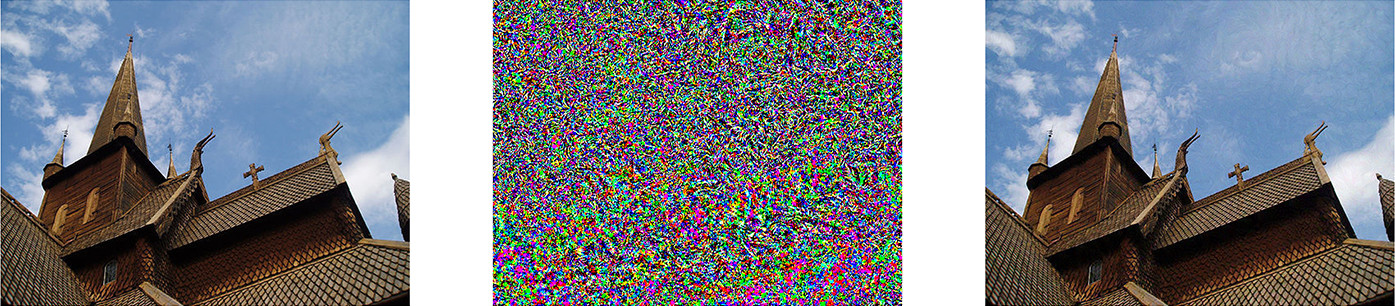
\includegraphics{{Plots/plots_base/adversarial_example_nocap.jpg}}
\caption{An adversarial example. The original Imagenette photograph on the
left is altered by adding the noise shown in the center (which is scaled up
to make it visible). The resulting image on the right appears identical to
the original, but is misidentified by the classifier.}
\label{example}
\end{figure*}
An adversarial example. The original Imagenette photograph on the left is
altered by adding the noise shown in the center (which is scaled up to make
it visible). The resulting image on the right appears identical to the
original, but is misidentified by the classifier.

\subsection{Attacks}

The FGSM attack \cite{goodfellow2014explaining} takes advantage of this
weakness in a straightforward manner. The attacker forms the perturbation
vector $\mathbf{\eta }$ to match the cost function gradient sign for a given
input, computing 
\begin{equation*}
\mathbf{\eta }=\epsilon _{\ast }\text{sign}(\nabla _{\mathbf{X}}J(\mathbf{%
\theta },\mathbf{X},y))
\end{equation*}%
where $\epsilon _{\ast }$ is the allowable level of perturbation, $J$ is the
network cost funtion, $\mathbf{\theta }$ is the vector of model parameters,
and $y$ is the true label. Thus, if the attacker is in posession of the
model and labeled training data, it is easy to train the network to behave
badly using simple backpropagation. The result is that the network will lose
certainty in the true label classification, and often misclassify the data
at random. The attack parameter $\epsilon _{\ast }$ may be scaled, of
course, but making $\epsilon _{\ast }$ much larger than the network
precision level $\epsilon $ may produce examples whose alteration is visible
to human reviewers, so smaller $\epsilon _{\ast }$ are desireable from the
adversarial perspective.

One can alter this attack to cause the network to favor a particular class
instead \cite{madry2020adversarial}. We will call this the Directed Gradient
Sign Method (DGSM). This time we use the loss function to direct the network
toward a specific desired label. We iterate using gradient descent for a
given number of iterations, and project the gradient onto the $l_{\infty }$%
-norm $\epsilon _{\ast }$-sphere, which has the effect of insisting that a
feature is not altered by more than $\epsilon _{\ast }$. For a given input $%
\mathbf{X}$, the attacker must solve the minimization problem 
\begin{eqnarray*}
\min_{\delta }\{J_{adv}(\mathbf{X}+\mathbf{\delta }) &=&J(\mathbf{\theta },%
\mathbf{X}+\mathbf{\delta },y_{desired}) \\
&&-J(\mathbf{\theta },\mathbf{X}+\mathbf{\delta },y_{true})\}\text{ } \\
\text{subject to }\left\vert \left\vert \mathbf{\delta }\right\vert
\right\vert _{\infty } &\leq &\epsilon _{\ast }
\end{eqnarray*}%
where $J$ is again the loss function, $\mathbf{\theta }$ the fixed network
parameters, $y_{desired}$ and $y_{true}$ are two different labels, and $%
\mathbf{\delta }$ is the directed perturbation vector. This requires using
forward passes and backpropagation within the network over $N$ iterations,
applying the update rule%
\begin{eqnarray*}
\mathbf{\delta }_{t} &=&\mathbf{\delta }_{t-1}-a\text{ sign}(\nabla L_{adv}(%
\mathbf{X}+\mathbf{\delta }_{t-1})), \\
\mathbf{\delta }_{t} &\leftarrow &\text{clip}(\mathbf{\delta }_{t},-\epsilon
_{\ast },\epsilon _{\ast })
\end{eqnarray*}%
begining with the zero vector $\mathbf{\delta }_{0}=\mathbf{0}$. The result
of this attack is that the classifier will incorrectly favor the chosen
label $y_{desired}$ in adversarial inputs, despite remaining perfectly
capable of correctly classifying unaltered inputs.

\subsection{Defences}

A theme that has emerged in the literature is that there is a strong
correlation between generally robust networks/inferencing and
networks/inferencing methods that are not easily swayed by adversarial
attacks. Of course, one also expects a cost in effort or accuracy to be
associated with increased robustness.

Our first defence we test is simply Perturbed Prediction Averaging. The
simple aim of this method is to "wash out" any adversarial perturbations by
averaging over many noisy predictions. This defence has the advantage that
it does not require retraining the network, and the only increased expense
is the cost of slower decisions at inference time. We predict the class for
each image based on an ensemble prediction for the original image and $N-1$
additional perturbed versions of the image, with the perturbations drawn
uniformly from the $\epsilon _{\max }$-ball in the $l_{\infty }$ sense
around the image, choosing $\epsilon _{\max }$ to be larger than any
expected adversarial alteration level $\epsilon _{\ast }$. For example, $%
\epsilon _{\max }$ can be set large enough that a uniform random $\left\vert
\left\vert \mathbf{\delta }\right\vert \right\vert _{\infty }\leq $ $%
\epsilon _{\max }$ perturbation would be easily noticed by a human. In that
case, we can assume that adversarial attacks will rely on $\epsilon _{\ast
}<<\epsilon _{\max }$. Using a modified softmax function, we can express the
probability for class $k$ of classes $\{1,2,...,K\}$ predicted using this
defense as%
\begin{equation*}
P(y_{k}\rvert \mathbf{X})=\frac{\sum_{i=1}^{N}e^{z_{k}(\mathbf{X}+\mathbf{%
\delta }_{i}\mathbf{)}}}{\sum_{j=1}^{K}\sum_{i=1}^{N}e^{z_{j}(\mathbf{X}+%
\mathbf{\delta }_{i}\mathbf{)}}},
\end{equation*}%
where $z_{j}(\mathbf{X}+\mathbf{\delta }_{i}\mathbf{)}$ is the output of the 
$j$th hidden node for a given network input $\mathbf{X}$ and with $\mathbf{%
\delta }_{i}=\mathbf{0}$, and $\left\vert \left\vert \mathbf{\delta }%
\right\vert \right\vert _{\infty }\leq \epsilon _{\max }$ for all $i$.

In practice we found that a choice of $\epsilon _{\max }=0.3($pixel range$)$
gave us perturbation that is easily noticeable. Of course, setting $\epsilon
_{\max }$ too high can lead to inaccurate classification results, since the
network was not trained on such noisy data; we must ballance the extent of
our defense with our practical needs.

On the other hand, there are many defensive measures that can be applied
directly to the neural network during training to allow faster inferencing
that is still adversarially robust. One method we explored is Adversarial
Training, where we generate adversarial examples that are added to the
training data for the network, either during the original training or during
a retraining step. Using FGSM examples is computationally efficient and
provides significant security improvements.

\section{Computational results}

\subsection{Resources}

Our computations were made using Jupyter Notebooks in Google Colaboratory
with their free GPU and TPU\ process time. All code and data interfaces are
available at the github address given above, in a manner optimized for
reproducibility.

\subsection{Imagenette data}

To keep our experiments within the scope of our resources, we used a subset
of the ImageNet dataset \cite{imagenet_cvpr09} called Imagenette\footnote{%
In keeping with the wishes of the dataset curators, we ask that you
internally read "Imagenette"\ with "a corny inauthentic French accent"
unless you are in fact a native French speaker, in which case you are asked
to render it in a similarly ridiculous American accent.} \cite{imagenette}
which includes only 10 out of the original 20k classes. These classes%
\footnote{%
The classes are as follows:\ \{tench (a fish), English terrier, cassette
player, chain saw, church, French horn, garbage truck, gas pump, golf ball,
parachute\}.} are selected to be as distinct as possible, with the intention
of allowing classifiers to reach high degrees of accuracy without extensive
training for more agile experimentation.

\subsection{Neural architectures}

After testing our attack strategy with smaller convolutional networks, we
performed the work for this paper by attacking and defending two standard
models used for image classification tasks, Wide ResNet and GoogLeNet. We
took advantage of pretrained PyTorch implementations of these models and
simply restricted the output to the ten classes of interest. While the
details of these architectures are outside the scope of this review, they
can be found in \cite{zagoruyko2016wide} and \cite{szegedy2015going}.

We retrained these networks with the output node layer corrected, using 5
epocs of stochastic gradient descent with a learning rate of 0.01 and
momentum value of 0.9. This base version of Wide ResNet achieved 99\%
accuracy on a test set of images, while GoogLeNet achieved 90\% accuracy.

\subsection{Creating Adversarial Examples}

\subsection{Defences}

\section{Analysis}

\section{Conclusions}

\bibliographystyle{amsplain}
\bibliography{acompat,JHU}

\end{document}
